\subsect{Sprint 9}{sprint9}

\underline{Fecha de inicio}: 11/02/2023

\underline{Fecha de fin}: 11/03/2023

\underline{Objetivos}:
\begin{itemize}
	\item Mejor implementación de las respuestas HTTP\@.
	\item \boldFont{Uso de un modelo de inteligencia artificial para la detección de imágenes inapropiadas.}
\end{itemize}

\underline{Descripción}:
Para este sprint se realizará un completo rediseño de la implementación de las respuestas HTTP, ya que se debe
facilitar su uso y la creación de nuevas respuestas en cada controlador.

El modelo de inteligencia artificial para la detección de imágenes inapropiadas
que se empleará en la aplicación se ha obtenido del repositorio de GitHub
\href{https://github.com/GantMan/nsfw_model}{\textit{GantMan/nsfw\_model}}~\cite{nsfw-model-repo}.
La implementación de este modelo se realizará en un nuevo servicio utilizando NodeJS y la librería TensorFlowJS\@.

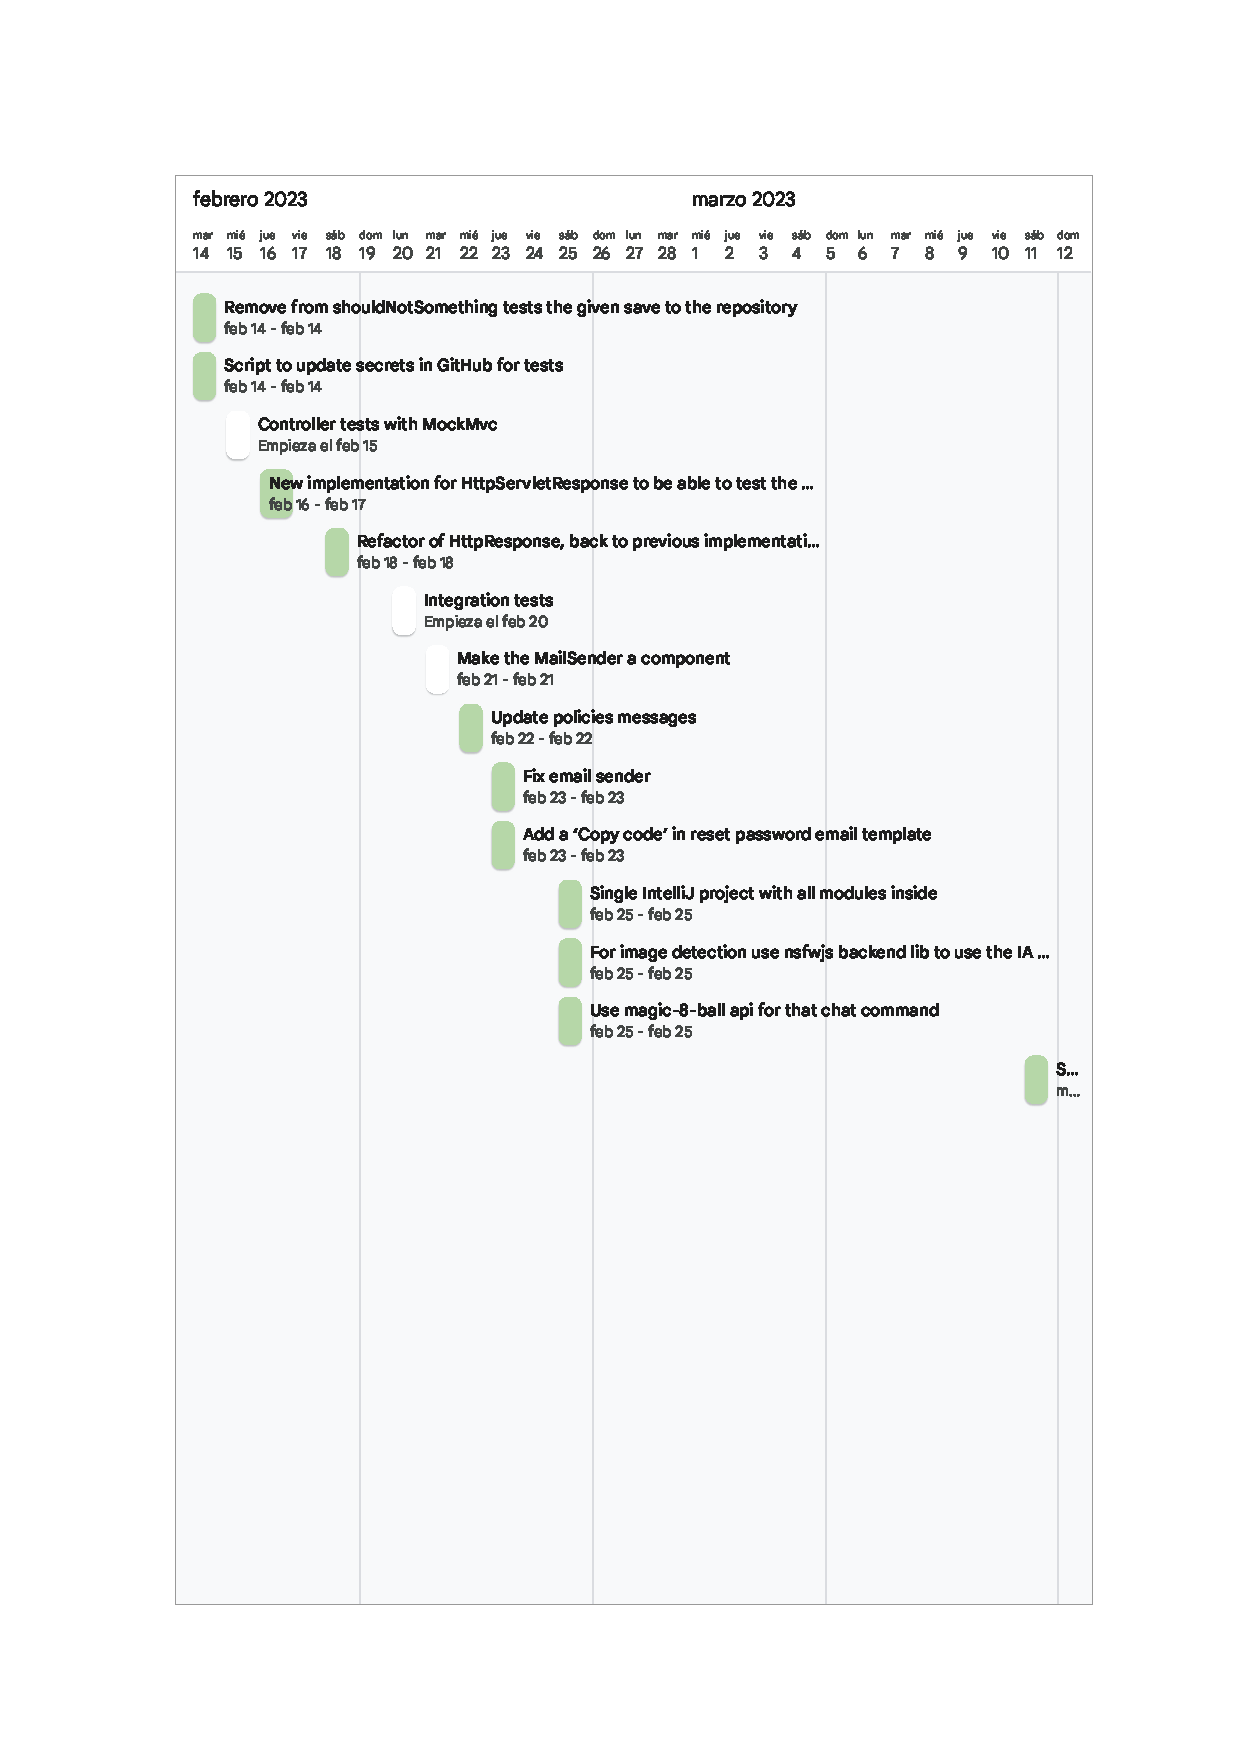
\includepdf[pages=-]{backlog/sprints/Sprint9.pdf}
